\documentclass[11pt,a4paper,landscape]{article}

\usepackage[utf8]{inputenc}
\usepackage[T1]{fontenc}
\usepackage[french]{babel}

\usepackage{styles/couleurs}
\usepackage{styles/boites}
\usepackage{styles/maths}
\usepackage{styles/figures}

\usepackage{amsmath}
\usepackage{amssymb}
\usepackage{graphicx}
\usepackage[most]{tcolorbox}
\usepackage{geometry}

\geometry{
  a4paper,
  landscape,
  left=8mm,
  right=8mm,
  top=6mm,
  bottom=6mm
}

\pagestyle{empty}
\setlength{\parindent}{0pt}
\setlength{\parskip}{0pt}

\begin{document}

% =========================================================
% TITRE
% =========================================================

\begin{center}
  {\sffamily\LARGE\bfseries\color{TitreC}
  Séquence 2 -- Théorème de Pythagore}\\[-0.05em]

  {\sffamily\large\bfseries\color{SavoirC}
  Activité 2 -- Le puzzle : suite -- Correction}
\end{center}

\vspace{-0.2em}

% =========================================================
% TROIS COLONNES
% =========================================================

\noindent
\makebox[\textwidth][c]{%

% =========================================================
% CAS 1
% =========================================================

\begin{minipage}[t]{0.315\textwidth}
\vspace{0pt}

\begin{tcolorbox}[
  enhanced,
  colback=ActionC!5,
  colframe=ActionC!55,
  boxrule=0.6pt,
  arc=2mm,
  left=2mm,
  right=2mm,
  top=1.5mm,
  bottom=1.5mm
]

\begin{center}

{\sffamily\bfseries\color{ActionC}
Cas 1}

\vspace{0.2em}

\[
AB=2{,}8\ \text{cm}
\qquad
AC=9{,}6\ \text{cm}
\]

\vspace{-0.6em}

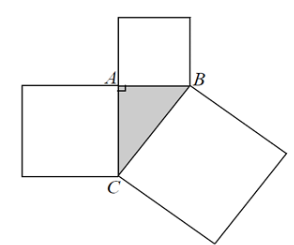
\includegraphics[
  width=0.72\linewidth,
  height=3.6cm,
  keepaspectratio
]{images/puzzle_original_triangle_carrés.png}

\vspace{-0.1em}

\textbf{Calculer \(BC\).}

\end{center}

\end{tcolorbox}

\vspace{0.15em}

\begin{tcolorbox}[
  enhanced,
  colback=white,
  colframe=NeutreC!35,
  boxrule=0.5pt,
  arc=1.5mm,
  height=7.6cm,
  left=3mm,
  right=3mm,
  top=2mm,
  bottom=2mm
]

\[
2{,}8\times2{,}8
=
7{,}84\ \text{cm}^2
\]

\[
9{,}6\times9{,}6
=
92{,}16\ \text{cm}^2
\]

\[
7{,}84+92{,}16
=
100\ \text{cm}^2
\]

\[
10\times10=100
\]

\[
\boxed{BC=10\ \text{cm}}
\]

\end{tcolorbox}

\end{minipage}

\hspace{5mm}

% =========================================================
% CAS 2
% =========================================================

\begin{minipage}[t]{0.315\textwidth}
\vspace{0pt}

\begin{tcolorbox}[
  enhanced,
  colback=ActionC!5,
  colframe=ActionC!55,
  boxrule=0.6pt,
  arc=2mm,
  left=2mm,
  right=2mm,
  top=1.5mm,
  bottom=1.5mm
]

\begin{center}

{\sffamily\bfseries\color{ActionC}
Cas 2}

\vspace{0.2em}

\[
AB=1{,}4\ \text{cm}
\qquad
AC=4{,}8\ \text{cm}
\]

\vspace{-0.6em}

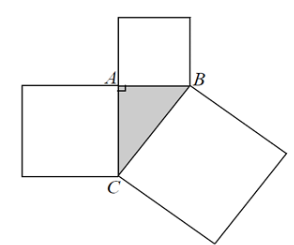
\includegraphics[
  width=0.72\linewidth,
  height=3.6cm,
  keepaspectratio
]{images/puzzle_original_triangle_carrés.png}

\vspace{-0.1em}

\textbf{Calculer \(BC\).}

\end{center}

\end{tcolorbox}

\vspace{0.15em}

\begin{tcolorbox}[
  enhanced,
  colback=white,
  colframe=NeutreC!35,
  boxrule=0.5pt,
  arc=1.5mm,
  height=7.6cm,
  left=3mm,
  right=3mm,
  top=2mm,
  bottom=2mm
]

\[
1{,}4\times1{,}4
=
1{,}96\ \text{cm}^2
\]

\[
4{,}8\times4{,}8
=
23{,}04\ \text{cm}^2
\]

\[
1{,}96+23{,}04
=
25\ \text{cm}^2
\]

\[
5\times5=25
\]

\[
\boxed{BC=5\ \text{cm}}
\]

\end{tcolorbox}

\end{minipage}

\hspace{5mm}

% =========================================================
% CAS 3
% =========================================================

\begin{minipage}[t]{0.315\textwidth}
\vspace{0pt}

\begin{tcolorbox}[
  enhanced,
  colback=ActionC!5,
  colframe=ActionC!55,
  boxrule=0.6pt,
  arc=2mm,
  left=2mm,
  right=2mm,
  top=1.5mm,
  bottom=1.5mm
]

\begin{center}

{\sffamily\bfseries\color{ActionC}
Cas 3}

\vspace{0.2em}

\[
BC=5{,}8\ \text{cm}
\qquad
AC=4{,}2\ \text{cm}
\]

\vspace{-0.6em}

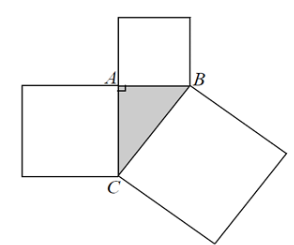
\includegraphics[
  width=0.72\linewidth,
  height=3.6cm,
  keepaspectratio
]{images/puzzle_original_triangle_carrés.png}

\vspace{-0.1em}

\textbf{Calculer \(AB\).}

\end{center}

\end{tcolorbox}

\vspace{0.15em}

\begin{tcolorbox}[
  enhanced,
  colback=white,
  colframe=NeutreC!35,
  boxrule=0.5pt,
  arc=1.5mm,
  height=7.6cm,
  left=3mm,
  right=3mm,
  top=2mm,
  bottom=2mm
]

\[
5{,}8\times5{,}8
=
33{,}64\ \text{cm}^2
\]

\[
4{,}2\times4{,}2
=
17{,}64\ \text{cm}^2
\]

\smallskip

\textbf{L'aire du petit carré est la différence entre
l'aire du grand carré et celle de l'autre carré.}

\[
33{,}64-17{,}64
=
16\ \text{cm}^2
\]

\[
4\times4=16
\]

\[
\boxed{AB=4\ \text{cm}}
\]

\end{tcolorbox}

\end{minipage}

} % fin du makebox

\end{document}